\chapter{Fundamentals} \label{fandamentals}
\label{chapter2}
In this chapter, we will delve into the foundational aspects of blockchain technology and P2P energy trading.
Initially, we will clarify the concept of a smart contract and explore its life cycle. Following that, we will introduce the most popular consensus mechanisms
and various blockchain platforms, examining their distinctions. Finally, we will outline the P2P energy trading paradigm,
drawing comparisons with traditional energy trading and we will explore different market clearing methods used on energy trading.

\section{Blockchain Technology}
A blockchain is a digital framework that functions as a decentralized, communal database. Within this framework, there exists an ever-expanding record of transactions
organized chronologically. Essentially, this digital structure operates much like a ledger, capable of housing digital transactions, data records, and executable code.
Transactions are grouped into larger units known as "blocks," each bearing a timestamp and cryptographic connections to prior blocks. This creates a linked sequence of records,
establishing the order of events within the blockchain. Beyond defining the data structure itself, the term "blockchain" is also widely used in academic literature to describe digital consensus
systems, algorithms or application domains that are constructed upon these foundational structures.\\
The primary objective of blockchain technologies is to eliminate the necessity for intermediaries and replace them with a distributed network of digital participants who
collaborate to authenticate transactions and preserve the ledger's integrity. In contrast to centralized systems, each member of the blockchain network maintains their own copy
of the ledger or can access it in the public cloud. Consequently, anyone within the network can access the historical record of system transactions and verify their legitimacy,
promoting a high level of transparency. With the removal of central management, the challenge lies in developing an efficient method to consolidate and synchronize multiple ledger
copies. The precise process of validation and ledger consolidation varies among different types of blockchains. However, in principle, network members compare their ledger versions
through a process resembling distributed voting, ultimately reaching a consensus on the valid ledger state. These validation mechanisms are commonly referred to as distributed
consensus algorithms.\\
\begin{figure}[h!]
    \centering
    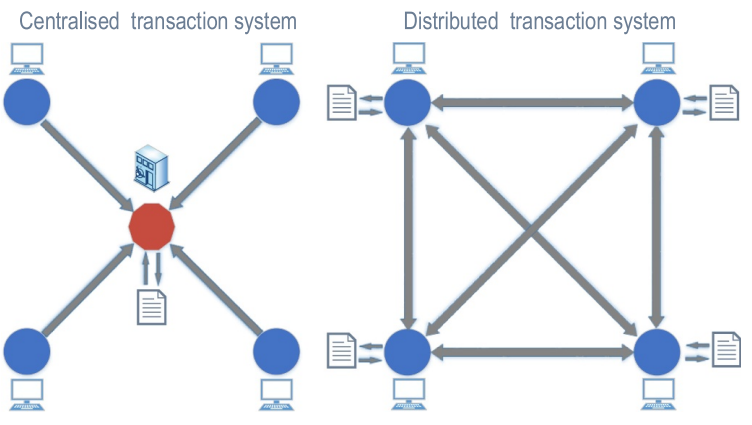
\includegraphics[scale=0.4]{Figures/centralised_vs_distributed.png}
    \caption{Centralized VS Distributed transaction systems \cite{andoni2019blockchain}}
\end{figure}\\
Blockchain also uses cryptographic techniques like hash functions and public-key cryptography to secure the ledger. Cryptographic hash functions are mathematical algorithms
or one-way processes that take an input and convert it into a specific-length output, such as a 256-bit string referred to as the hash output. Their effectiveness relies on the
extreme difficulty of recreating the original input data from the hash output alone, ensuring collision resistance. Furthermore, blockchain employ public-key cryptography, an
asymmetric cryptographic system where each user possesses two cryptographic keys, comprised of numeric or alphanumeric characters:
\begin{itemize}
    \item A secret private key
    \item And a public key which can be shared with other network users
\end{itemize}
These keys are mathematically interconnected, permitting information encrypted with one key to be decrypted exclusively by its counterpart. This public-private key cryptography
ensures:
\begin{itemize}
    \item Authentication: The network can verify the sender's identity because only the sender's public key can decrypt the initial message, which is encrypted and digitally signed
          using the sender's private key
    \item Verification that a transaction originates from the claimed source. Messages processed with a recipient's public key can only be decrypted by the intended recipient possessing
          the corresponding private key.
    \item And authorization, confirming that actions are executed by users with the appropriate privileges
\end{itemize}
These security measures, along with other standard communication features such as data integrity and confidentiality, are achieved within blockchain systems through peer-to-peer
communication and advanced cryptographic techniques. \cite{andoni2019blockchain}

\subsection{Smart Contracts}
Blockchain can also be paired with smart contracts, realizing fully their potential. Smart contracts are executable programs capable of modifying a ledger automatically when specific
conditions are fulfilled, often related to honoring agreements between parties. These contracts encode legal terms and constraints in a computer-readable language. They are
self-enforcing and tamper-resistant, eliminating the need for intermediaries and reducing transaction-related costs. \cite{andoni2019blockchain} \\
The life cycle of a smart contract, consists of 4 main phases: \cite{ZHENG2020475}
\begin{enumerate}
    \item Creation of smart contract: Multiple parties negotiation on the rights, obligations and prohibitions of their contract. They reach a common agreement and a smart contract is
          build. The smart contract development is done using a smart contract programming language compatible with the blockchain that will be deployed. The smart contract need to be tests
          vigorously as logical code mistakes could result into a breach of the agreement between the parties and assets could be in danger.
    \item Deployment of smart contract: The contract is deployed on a blockchain platform and can't be modified due to the immutability of the blockchain. The contract can be accessed
          by the parties through the blockchain platform. They can initiate the different actions coded by the contract, like for example locking an amount of digital tokens into the contract
          until a condition is met.
    \item Execution of smart contract: The smart contract in effective, the contract conditions are evaluated and the contract statements are executed when the conditions are met.
    \item Completion of smart contract: After the execution of the smart contract new states of all involved parties are updated and stored in the blockchain. At this stage the digital
          assets are moved between the parties based on the initial agreement.
\end{enumerate}
\begin{figure}[h!]
    \centering
    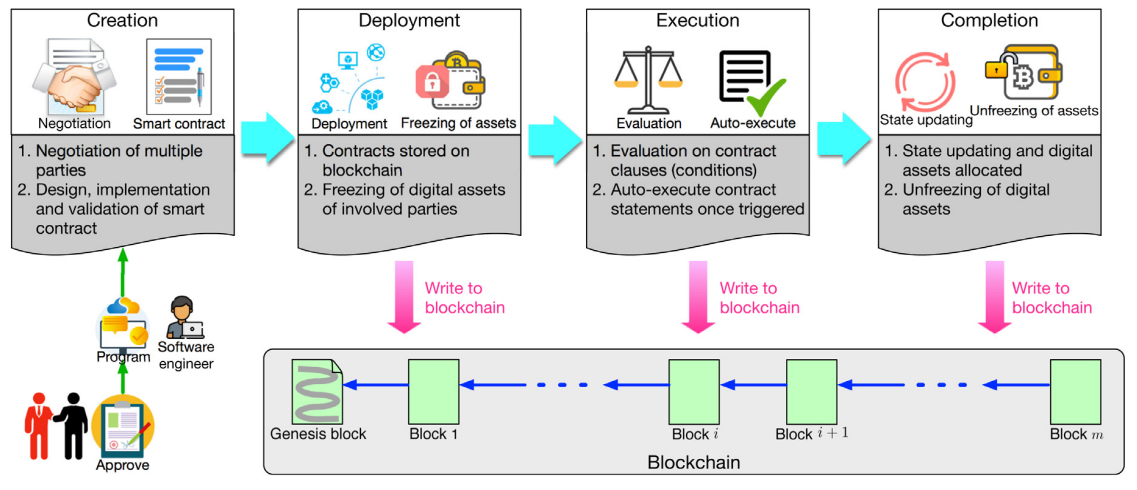
\includegraphics[scale=0.5]{Figures/smart_contract_life_cycle.png}
    \caption{LifeCycle of a smart contract \cite{ZHENG2020475}}
\end{figure}
The main challenge with the creation of a smart contract comes from the fact that blockchains are immutable. As soon as a contract is deployed on the blockchain it can't be modified.
This is a big challenge for smart contract developers as they need to be sure that everything is going to work as expected from the first try.
So it's very important to perform extensive functional tests on the smart contract code before its deployment. \cite{ZHENG2020475}


\subsection{Public and private blockchain networks}
A blockchain network or system can adopt various rules and system architectures based on its intended functionality and specific use cases. Typically, blockchain systems comprise of
network users and validators. User nodes have the capability to initiate or receive transactions and maintain a copy of the ledger. Validators, in addition to read access privileges,
are tasked with approving ledger modifications and achieving consensus across the network concerning the ledger's valid state. Depending on the system's configuration, there may be
partial or universal access rights and validation rights.\\
Public blockchain systems are open to all internet users, while private blockchains restrict access to authorized participants only. Permissionless ledgers are fully decentralized
and resistant to censorship, allowing any network member to participate in transaction validation. Conversely, permissioned ledgers grant write access rights to specific validator
nodes, making the ledger modification process more controlled. In public and permissionless ledgers, users and validators have no prior knowledge of each other, relying on
game-theoretic equilibria and rewards to encourage collaborative and trustworthy ledger management. This incentive structure often involves the expenditure of resources, such as
computational power, electricity, or penalties, to discourage selfish behavior \cite{andoni2019blockchain} Examples of public blockchains with a permissionless ledger are Bitcoin created by Satoshi Nakamoto
\cite{Nakamoto} and Ethereum which was the first public blockchain that made use of smart contracts, proposed by Vitalik Buterin \cite{wood2014ethereum}.\\
Private and permissioned ledgers, on the other hand, operate with known user identities, similar to "know-your-customer" (KYC) practices. Validator nodes are recognized and trusted
to act honestly, eliminating the need for artificial incentives to ensure system operation. Consequently, private and permissioned ledgers can offer increased speed, flexibility
and efficiency, although this comes at the cost of reduced immutability and censorship resistance \cite{andoni2019blockchain}. The most popular permissioned blockchain is Hyperledger fabric proposed by IBM
\cite{androulaki2018hyperledger}.\\
\begin{table}[h!]
    \centering
    \begin{tabular}{l|ll}
        \textbf{Aspect}  & \textbf{Public Blockchain} & \textbf{Private Blockchain}     \\
        \hline
        Access Control   & Open to anyone             & Restricted access               \\[5pt]
        Permission Level & Permissionless             & Permissioned                    \\[5pt]
        Consensus        & Mainly PoW \& PoS          & Various consensus mechanisms    \\[5pt]
        Participants     & Anyone can join            & Approved participants           \\[5pt]
        Privacy          & Anonymous/Pseudonymous     & Known identities (KYC)          \\[5pt]
        Performance      & Slower due to open access  & Faster due to restricted access \\[5pt]
        Scalability      & Limited                    & Potentially better              \\[5pt]
        Example          & Bitcoin, Ethereum          & Hyperledger Fabric              \\[5pt]
    \end{tabular}
    \caption{Public versus private blockchains}
\end{table}

\subsection{Blockchain consensus mechanisms}
In this section, we will present some mechanisms used by blockchain technologies to achieve consensus.
\subsubsection{Proof of Work (PoW)}
The idea behind PoW, as used in Bitcoin, comes from 'Hashcash' which was created to prevent internet resources from being overwhelmed by denial of service attacks.
In PoW, validators or miners compete to add a new block to the existing blockchain by solving a puzzle. They do this by generating a hash that begins
with a certain number of zeros. To achieve this, they add a unique random number (nonce) to the block and calculate the hash of the block's information. This information
includes details like the previous block's hash and a special hash for all the transactions in the block (Merkle tree). Every miner's goal is to produce a hash that's
lower than a specific target value. Since miners can't predict or control the outcome, they have to try different combinations until they succeed. This process requires more
and more computational power as you need more leading zeros. When a miner finally finds the hash that is less than the target, the block is added to the Bitcoin network. Other
nodes check to make sure the transactions are valid and if they are, they accept the newly created block of transactions and the successful miner gets a financial reward.
\cite{andoni2019blockchain}

\subsubsection{Proof of Stake (PoS)}
Proof of Stake, differs from traditional systems by replacing computational work with a random selection method. In PoS, the likelihood of successfully mining a block is
directly linked to the wealth of the validators. The chances of creating a block depend on how much cryptocurrency the nodes have invested in the system, essentially their
coin ownership. This approach potentially allows for faster blockchains with significantly lower electricity consumption and a reduced risk of a 51\% attack.
Unlike other systems, PoS doesn't require the constant creation of new coins to motivate validators. Instead, miners can be rewarded solely with transaction fees, making it
less advantageous to invest heavily in specialized hardware like ASICs.
PoS can also utilize game-theoretical mechanisms to discourage collusion and centralization, often penalizing dishonest or malicious behavior. However, PoS systems face a
primary vulnerability known as the 'nothing at stake' problem. This means that validators can easily vote or claim financial rewards on multiple chains without significant cost.
To address this, various solutions have been proposed, including penalties for validators who create blocks on multiple chains and automatic deductions of owned or deposited
coins. Another approach is to punish validators for creating blocks on the wrong chain, similar in concept to PoW, where validators also incur the cost of electricity.
The latter approach exposes validating nodes to greater risks, but it doesn't require them to be known in advance.
\cite{andoni2019blockchain}

\subsubsection{Practical Byzantine Fault Tolerance (PBFT)}
Byzantine Fault Tolerance (BFT) algorithms find their roots in the study of Byzantine faults, which was initially outlined by Lamport and his colleagues in a significant
computer science paper. To put it simply, this issue revolves around a group of Byzantine generals, or in the context of blockchain, nodes, trying to come to an agreement on
a coordinated course of action. Imagine these generals needing to synchronize their different army units to attack a fortress simultaneously (in the blockchain context, this
means reaching a consensus on whether to validate a block or a set of transactions).
The problem arises because the messages exchanged between these generals must travel through enemy territory, where they could get lost without anyone knowing (think of this
as an unreliable, distributed network). Additionally, some of these generals might be traitors with a vested interest in disrupting the battle plan. They might send false or
distorted messages, or simply not respond to messages at all. The main challenge is to make sure that the loyal generals can agree on the attack plan despite this, and that a
small number of traitors don't lead them to adopt a flawed plan.
In blockchain terms, this means that even if there are a few untrustworthy or potentially malicious nodes, they shouldn't be able to force the validation of a bad block or a
set of transactions.\\
A practical approach for Byzantine Fault Tolerance was introduced by Castro and Liskov \cite{castro1999practical}, for achieving Byzantine Fault Tolerance (BFT) with minimal
computational overhead. Their approach, known as Practical Byzantine Fault Tolerance (PBFT), introduces the concept of primary and secondary replicas. In PBFT, secondary
replicas are responsible for verifying the accuracy and responsiveness of the primary replica and can take over as the new primary if the original primary becomes compromised.\\
PBFT is better suited for use with trusted environment rather than public permissionless ledger. Transactions are signed and verified by known validator nodes and they are
considered valid when a sufficient amount of signatures is reached ans thus also consensus is reached.
\cite{andoni2019blockchain}

\subsubsection{Proof Of Authority (PoA)}
Proof of authority consensus algorithm relays on one or a group of peers to generate new blocks for the network. Network participants holding a special key are responsible to
for generating all network blocks. If the majority of all peer with the special key sign a block, then it's getting accepted into the network. So the network is putting their
trust to a group of authorized peers to generate and validate new blocks. The validators could be elected by a network vote and could be also possible to add new validators with
the same mechanism.
\cite{andoni2019blockchain}

\subsubsection{Comparison of popular consensus mechanisms}

In the table below we compare the different properties of the consensus mechanisms we analyzed in the section above.
Please note that for PoW, 51\% of hash power is regarded as the threshold for one to gain control of the network
but selfish mining strategy in PoW systems could help miners to gain more revenue by only 25\% of the hashing power and thus
the tolerated power of adversary is considered to be 25\%.
\begin{table}[h!]
    \centering
    \begin{tabular}{l|llll}
        \textbf{Aspect}    & PoW            & PoS                & PBFT \& variants   & PoA                \\
        \hline
        Node identity      & Permissionless & Both cases         & Permissioned       & Permissioned       \\
        management         &                &                    &                    &                    \\[5pt]
        \hline
        Energy consumption & High           & Low                & Moderate           & Low                \\[5pt]
        \hline
        Node scalability   & $> 1000$       & $> 1000$           & $< 100$            & $< 100$            \\[5pt]
        \hline
        Transactions per   & 7-30           & 100-200            & up to 110k         & High               \\
        second             &                &                    &                    &                    \\[5pt]
        \hline
        Tolerated power    & $< 25\%$*      & $< 51\%$           & $< 33.3\%$         & $< 51\%$           \\
        of the adversary   & comput. power  & stake              & replicas           & of validators      \\[5pt]
        \hline
        Security           & High           & Depended on        & High within known  & Relied on approved \\
                           &                & participants stake & participants       & authorities        \\[5pt]
        \hline
        Example            & Bitcoin        & Ethereum           & Hyperledger Fabric & VeChain            \\[5pt]
    \end{tabular}\\
    \caption{Comparison of popular consensus algorithms \cite{blockchainTech}}
\end{table}

\pagebreak
\subsection{Blockchain Platforms}
In this section we analyze different available blockchain platforms. Each of the blockchain platforms have different architectures but all of them try to achieve
three main goals:
\begin{itemize}
    \item \textbf{Decentralization}: How censorship resistant is the network, not being able to be controlled or influenced significantly by a small group of network participants.
    \item \textbf{Security}: How secure and robust is the network against attacks from bad actors.
    \item and \textbf{Scalability}: The ability to process transactions, store data and reach consensus as more users are added to the network.
\end{itemize}
It is very difficult to have an architecture that fully achieves these three goals simultaneously. Different approaches improve on two
of the goals in expense of the third. For example, Bitcoin achieves great security and decentralization but it lacks in terms of scalability.

\subsubsection{Bitcoin}
Bitcoin is a public and permissionless blockchain platform that uses the PoW consensus mechanism. Bitcoin protocol makes use of the unspent transaction output (UTXO) model.
In the UTXO model, each transaction has one or more inputs and outputs. The inputs specifies the assets involved in the transaction which must come from a previous transaction output that has not been utilized
in any prior transactions. Meanwhile, the output component is responsible for transferring these assets to a new address. The UTXO model serves a crucial role within the blockchain ecosystem by allowing
network nodes to track the origin of assets involved in any given transaction. This enables them to verify whether the party initiating the transaction possesses the legitimate right to spend those assets.
The movement of assets is recorded in a directed acyclic graph (DAG) between addresses.\\
UTXOs can be owned not only by public keys but also by scripts expressed in simple stack-based programming language. The script requests the data that satisfies the script from a transaction that tries to
spend the UTXO owned by the script. The bitcoin scripting language is not Turing-complete and thus it has limited capabilities not allowing the execution of complex smart-contracts.
\cite{blockchainTech,wang2017novel}
\begin{figure}[h!]
    \centering
    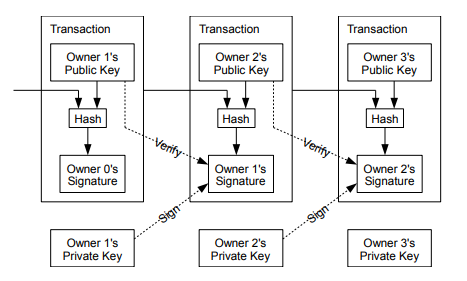
\includegraphics[scale=0.8]{Figures/bitcoin_transactions.png}
    \caption{Bitcoin transactions schematic \cite{Nakamoto}}
\end{figure}\\
Bitcoin network participants can choose to be either clients or miners. Clients are able to send and receive transactions while miners are in charge of creating new blocks through the PoW consensus mechanism.
All network participants keep a copy of the blockchain containing all the recorded transactions and can verify at any time the validity of a transaction.
Transactions are transmitted to the neighboring network peers and are propagated through the network. If the transaction is found to be invalid, it is not broadcasted further to the network and the propagation
stops. Miners store the incoming transaction in a transaction pool if they are valid. A block is constructed out of the transactions in the pool up to the upper block size limit which is about 1 MB. In a UTXO
transactions the input amount can be greater that the output one leaving the rest of the amount as a fee to the miners incentivizing them to prioritize the inclusion of the transaction in the next block.
\cite{blockchainTech,wang2017novel,Nakamoto,UTXOvsACCOUNT}

\subsubsection{Ethereum}
Ethereum is also a public and permissionless platform designed to build and use decentralized applications that run smart contracts. Ethereum smart contracts are written in a fully-fledged Turing-complete programming
language (named Solidity). An Ethereum virtual machine (EVM) is hosted on each network node which is used for the execution of smart contracts. Ethereum was initially relying on the PoW consensus mechanism for the creation of new blocks but it was
later transitioned in PoS.\\
Ethereum uses the account based transaction model where a global ledger is stored and maintained by all network parties based on the PoS consensus. Each block of the blockchain represents a different state of the ledger, this
allows everyone to go through the states of the ledger and validate the origin an legitimacy of a transaction.\\
There are three different account types in Ethereum:
\begin{itemize}
    \item \textbf{Contract Accounts}: A contract account is controlled by code executed by the EVM. They can create transactions with addresses stored in the contract or other contract accounts.
    \item \textbf{Externally Owned Accounts}: These accounts can initiate transactions to transfer Ether to other externally owned accounts, create new contracts or execute functions of existing contract accounts.
    \item \textbf{Miners/Stakers}: They collect unverified transactions, compute a valid state of the ledger, validate transactions, verify signatures and execute code. They collect transactions from the unverified transactions
          pool and compute a new state for the ledger for the next blockchain block choosing transactions based on the fee included in them. They higher the fee the higher the incentive to choose a transaction.
\end{itemize}
When we refer to Ethereum we refer to the open and public Ethereum blockchain network although the Ethereum software is open source and can be also used to create a private blockchain network.
\cite{blockchainTech,ethereum,UTXOvsACCOUNT}

\begin{figure}[h!]
    \centering
    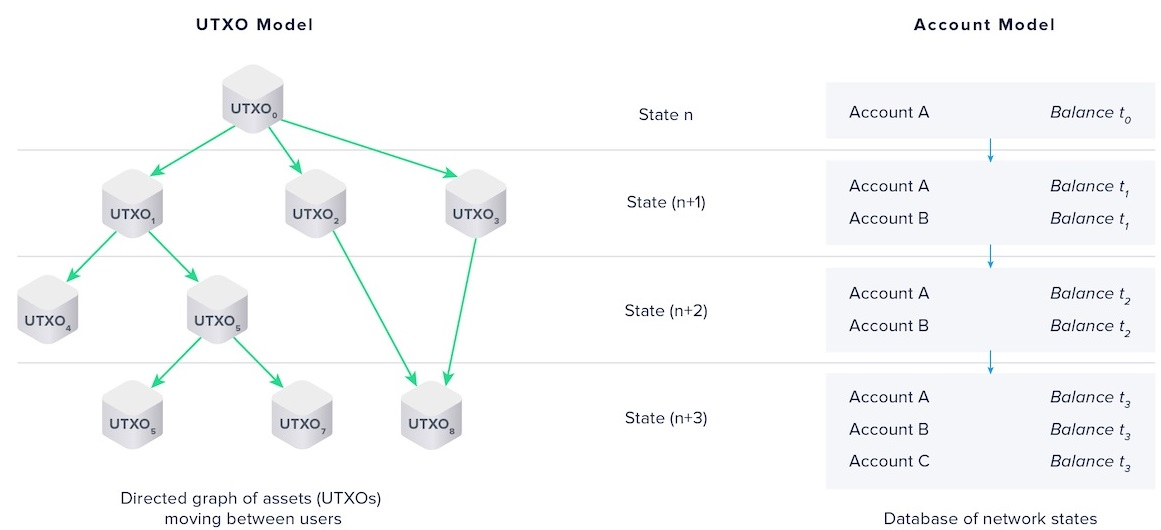
\includegraphics[scale=1.2]{Figures/utxo_vs_account_model.jpg}
    \caption{UTXO VS Account Model \cite{UTXOvsACCOUNT}}
\end{figure}

\subsubsection{Hyperledger}
Hyperledger is an open-source, global ecosystem of enterprise-grade blockchain technologies hosted by The Linux Foundation.
Hyperledger frameworks are designed for permissioned blockchain applications and parties need to be authorized to join the network.
In the hyperledger architecture, the following components are defined:
\begin{itemize}
    \item Consensus Layer: Verify blocks of transactions and agree on the order.
    \item Smart Contract Layer: Processes transactions
    \item Communication Layer: Handles the P2P transport
    \item Data Store Abstraction: Handles different data-stores
    \item Crypto Abstraction: Handles cryptographic algorithms
    \item Identity Service: Registers and authenticates identities of the network
    \item Policy Service: Responsible for policy management
    \item APIs for interaction with other applications
    \item Inter-Operation service: Handles the inter-operation with other blockchain networks
\end{itemize}
Different Hyperledger frameworks have been constructed based on the Hyperledger architecture.
One of the most popular Hyperledger platforms is Hyperledger Fabric.\\
Fabric functions as a distributed operating system designed for permissioned blockchains, running distributed applications that are
coded in widely used programming languages like Go, Java, and Node.js. It maintains a secure record of
its execution history using an immutable replicated ledger data structure, all while lacking any
integrated cryptocurrency. In Fabric, smart contracts are called as Chaincodes and reading or writing the ledger is an operation referred to as a "proposal".
Distributed application within Fabric consists of chaincodes.
A chaincode contains the program code responsible for implementing the application's logic and operates during the execution phase.
Chaincode represents the central element of a distributed application in Fabric and may be authored by a developer whose trustworthiness
is not guaranteed. There are specific chaincodes designed for managing the blockchain system and overseeing
parameters, collectively referred to as system chaincodes.
Fabric nodes can have one of the three roles below:
\begin{itemize}
    \item Client: Submit transaction proposals for execution.
    \item Peers : Execute transaction proposals and validate transactions. All peers has a copy of the blockchain ledger.
          Not all peers can execute all transaction proposals, only endorsing peers can. Execution of a chaincode depends on it's endorsement policy,
          which defines what peers and how many of them can validate it.
    \item  Ordering Service Nodes (OSN): The ordering service receives transactions from all channels in the network, orders them chronologically
          on a per-channel basis, and packages them into blocks. The blocks will be delivered to peers on the channel for final
          validation and commitment. This design choice renders consensus in Fabric as modular as possible and simplifies the replacement
          of ordering service nodes.
\end{itemize}
In a private Fabric network, participants usually reach consensus through the PBFT mechanism.
\cite{blockchainTech,hyperledger}

\pagebreak
\subsubsection{Comparison between blockchain platforms}
In this section we collected all the main differences between the three popular blockchain platforms analyzed above.
In the following table the main characteristics of a blockchain platform are presented along with how each characteristic compares
between the three popular platforms.
\begin{table}[h!]
    \centering
    \begin{tabular}[rounded-corners]{l|lll}
        \textbf{Aspect}         & \textbf{Bitcoin}     & \textbf{Ethereum}          & \textbf{Hyperledger Fabric} \\
        \hline
        Purpose                 & Digital Currency     & Decentralized Apps         & Enterprise blockchain       \\[5pt]
        Target Audience         & Individuals          & Developers, Individuals    & Enterprises, consortiums    \\[5pt]
        Permission Restrictions & Permissionless       & Permissionless             & Permissioned                \\[5pt]
        Access to data          & Public               & Public \& Private          & Private                     \\[5pt]
        Consensus               & PoW                  & PoS                        & PBFT                        \\[5pt]
        Transaction Speed       & Slow (~7/sec)        & Faster (~15-30/sec)        & Moderate speed              \\[5pt]
        Native Currency         & Bitcoin              & Ether                      & None                        \\[5pt]
        Scripting               & Not Turing-Complete, & Turing-Complete,           & Turing-Complete,            \\
                                & Limited Stack-based  & High-Level language        & High-Level languages        \\
                                & scripting            & Solidity                   & Go, NodeJS, Java            \\[5pt]
    \end{tabular}
    \caption{Comparison of popular blockchain platforms}
\end{table}

\subsection{Trusted Authorities}
Blockchain strives for a trustless and decentralized system but there are some aspects that still require some kind of a trusted authority to operate. Such 
example is the bridging of off-chain and on-chain data. A blockchain network has only access to what already exists in the blockchain and is completely isolated. 
In order to bridge off-chain data into the blockchain network, some kind of a trusted authority in needed. Such trusted authorities are also called oracles. Their 
responsibility is to retrieve, verify and feed off-chain data into the blockchain network which can then be used by decentralized applications. Another example of trusted
authority in the blockchain network, is a group responsible of bridging off-chain assets into the blockchain network in the form of a token. Such assets could for example
be a real world currency. The simplest way to achieve this is to store and lock the real world currency (effectively, moving it out of circulation) and minting the relevant amount
of a corresponding token into the blockchain network. With the opposite procedure they can then lock the corresponding blockchain network token and unlock the real world asset.
In general a trusted authority is a middle man that bridges real world data or assets into the blockchain network. The role of a trusted authority can sometimes be replaced by 
algorithms but with a cost on complexity and possibly security of the solution. \cite{oracles}\cite{stablecoins}

\section{P2P Energy Trading}
Energy generation by prosumers can be unpredictable due to different variables which makes it difficult to predict.
Such variables could be the amount of sun for PV units or the wind speed for wind turbines.
In case of energy surplus, a prosumers has three possible options:
\begin{itemize}
    \item To store the energy in batteries considering there is capacity left
    \item Export the excess energy to the electricity grid in market prices
    \item Or sell it to another energy consumer
\end{itemize}
I case of the P2P energy trading model, consumers and prosumers are buying and selling energy directly among them,
on a local energy market, formed by the ask and offered energy prices. In such a local energy trading
market, the network participants first share their generated energy locally and then
trade with the retailers. The local market prices are typically set between the export energy price,
which is the prices the prosumers are selling to the retailers and the retail price, which is the price to buy energy from
retailers. In this way, both prosumers and consumers are benefiting as the former sell energy in a better price while the
latter buy cheaper energy. \cite{Soto2021}

\begin{figure}[h!]
    \centering
    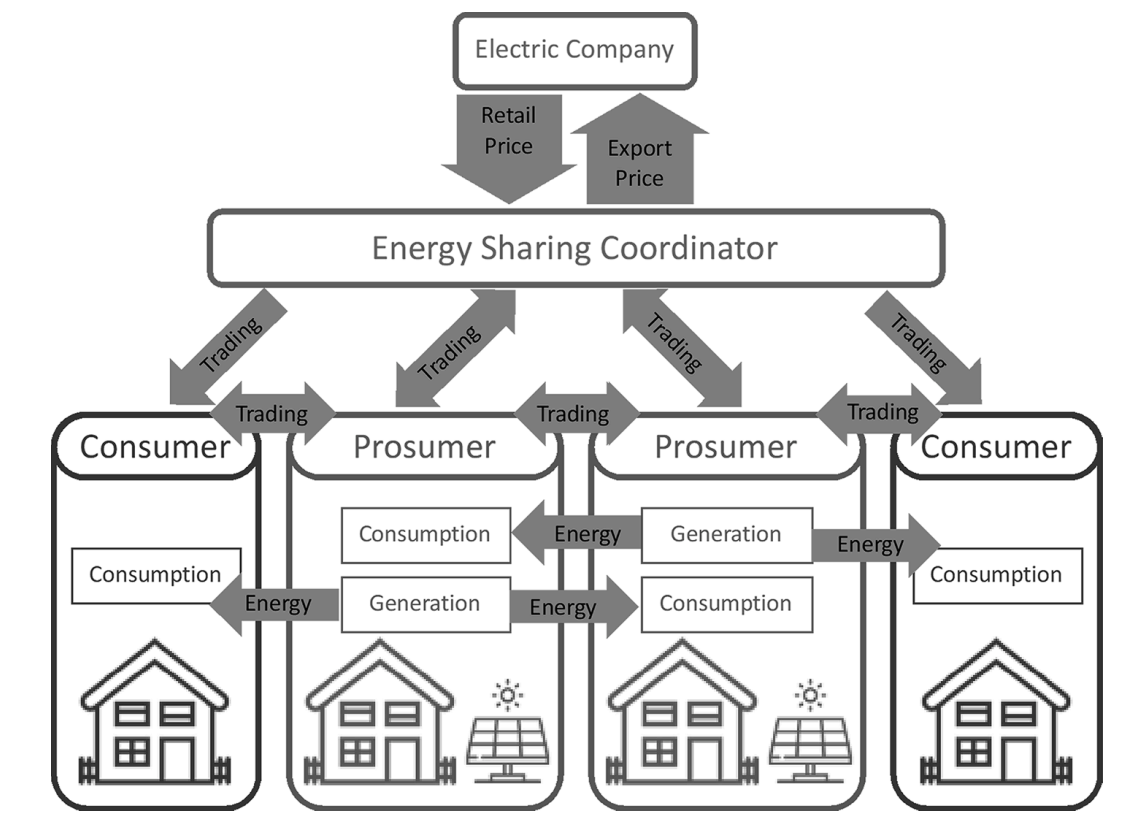
\includegraphics[scale=0.4]{Figures/P2P_Energy_Trading_Model.png}
    \caption{P2P energy trading model \cite{Soto2021}}
\end{figure}

\subsection{Conventional versus P2P energy trade}
In this section, we will discuss what are the benefits of P2P energy trade, what its limitations
and how it compares against the conventional energy trading model. Conventional energy trading is usually one-way,
energy is transmitted from large-scale generators to consumers while cash flow is the other way around, from consumers to
energy providers. The market price can not be influenced directly from the consumers and it is set by energy providers based on market
conditions. In contrast, P2P energy trade is a multi-directional procedures where both the energy and cash, flow between prosumers
and prosumers. The energy price is set by the microgrid based on the participants' bids.
P2P energy trading will also have some impact on the community. It creates new job opportunities for the maintenance and operation
of the P2P systems, it increases social trust as the community works together for their energy needs and generally it creates a great
attachment to the community as the participants have a direct connection with each other. \cite{Soto2021}
\begin{table}[h!]
    \begin{tabular}[rounded-corners]{l|ll}
        \textbf{Aspect} & \textbf{P2P Energy Trade}             & \textbf{Conventional Energy Trade}  \\
        \hline
        Transparency    & High transparency in pricing,         & Less transparent, prices may be     \\
                        & sources and transactions              & influenced by not easily traceable  \\
                        &                                       & sources                             \\[5pt]
        Innovation and  & Relies on blockchain, smart contracts & More traditional infrastructure,    \\
        Technology      & and IoT devices for trading           & slower to adapt new technologies    \\ [5pt]
        Environmental   & Emphasizes renewable energy           & May or may not prioritize           \\
        Impact          & usage, sustainability and             & renewable energy sources            \\
                        & local energy production               & and sustainability                  \\[5pt]
        Regulatory      & Can face hurdles dut to evolving      & Compliance with energy policies     \\
        Challenges      & energy market regulations             & and regulations is more established \\[5pt]
        Scalability and & Can be more scalable, efficient and   & May face challenges in adapting to  \\
        Efficiency      & adaptable to localized energy needs   & rapid changes or catering to        \\
                        &                                       & localized demands                   \\[5pt]
    \end{tabular}
    \caption{P2P versus Traditional energy trading}
\end{table}

\subsection{Microgrid Markets}
Apart from the physical connections of a microgrid, there is also a market layer where all the participants' transactions happen.
A microgrid market is usually classified by three main processes :
\begin{itemize}
    \item Identity verification: Verifies the identity of the participant and confirms that he/she can participate in the microgrid market.
    \item Market opening: At market opening, sellers and buyers can submit their bids and the market automatically completes the transactions
          and does the price matching based on the trading rules.
    \item Market closing: The market closes and the participants can't submit any bids until it opens again \cite{wang2017novel}
\end{itemize}

In the following subsections, different market clearing methods will be presented.

\subsubsection*{Continuous Double Auction (CDA)}
Most P2P trading platforms are making use of the continuous double auction design for their market layer.
In a CDA market, buyers and sellers can submit their bids at any time of the trading period and
market clears continuously. Buyers' bids are ordered in a descending order, from highest to lowest,
while sellers' bids from lowest to highest. Then a "price first and time first" principle is applied
and the orders are cleared based on the given bids. A CDA market order book example can be seen on the table below. \cite{wang2017novel,DeTrade}

\begin{table}[h!]
    \begin{minipage}[c]{\textwidth}
        \centering
        \begin{tabular}{|c|c|c|c|c|c|}
            \hline
            \multicolumn{6}{|c|}{\textbf{Order Book Before Clearing}}                                                                                               \\
            \hline
            \multicolumn{3}{|c|}{\textbf{Buy Orders}} & \multicolumn{3}{|c|}{\textbf{Sell Orders}}                                                                  \\
            \hline
            Buyer                                     & Requested Price                            & Provided energy & Seller & Requested Price  & Requested energy \\
                                                      & units per energy                           & energy units    &        & units per energy & units            \\
                                                      & unit                                       &                 &        & unit             &                  \\
            \hline
            B1                                        & 10,5                                       & 5               & S1     & 10,2             & 3                \\
            B2                                        & 10,0                                       & 3               & S2     & 10,5             & 1                \\
            B3                                        & 9,9                                        & 4               & S3     & 10,8             & 4                \\
            B4                                        & 9,8                                        & 5               & S4     & 11,1             & 3                \\
            \hline
        \end{tabular}
    \end{minipage}\\
    \begin{minipage}[c]{\textwidth}
        \centering
        \begin{tabular}{|c|c|c|c|c|c|}
            \hline
            \multicolumn{6}{|c|}{\textbf{Order Book After Clearing}}                                                                                                \\
            \hline
            \multicolumn{3}{|c|}{\textbf{Buy Orders}} & \multicolumn{3}{|c|}{\textbf{Sell Orders}}                                                                  \\
            \hline
            Buyer                                     & Requested Price                            & Provided energy & Seller & Requested Price  & Requested energy \\
                                                      & units per energy                           & energy units    &        & units per energy & units            \\
                                                      & unit                                       &                 &        & unit             &                  \\
            \hline
            B1                                        & 10,5                                       & 1               & S3     & 10,8             & 3                \\
            B2                                        & 10,0                                       & 3               & S4     & 11,1             & 1                \\
            B3                                        & 9,9                                        & 4               &        &                  &                  \\
            B4                                        & 9,8                                        & 5               &        &                  &                  \\
            \hline
        \end{tabular}
    \end{minipage}
    \caption{Order book in CDA market, before and after clearing}
\end{table}

The higher bid of a buyer is called the outstanding bid while the higher bid of a seller is called outstanding ask. When the outstanding bid is less or equal to the outstanding
ask, a transaction is happening with the transaction price being equal to the average of the two prices. This process continues until there the outstanding bid is more than the
outstanding ask. This process is called one round of transactions and at least one transaction occurs during that process. In the above table we can see that one round of transactions
is performed which includes two transactions, the one between B1 and S1 for 3 energy units and the one from B1 to S2 for 1 energy unit. \cite{wang2017novel}

\subsubsection*{Time Descrete Double Auction (TDDA)}

In a TDDA market, transaction happens at discrete time intervals rather than continuously. Specific time intervals are specified when the participants can make their buying or selling
bids. At the end of this time interval, the system matches buy and sell order based on the outstanding bids and the outstanding asks, like the CDA market. TTDA is more or less and
extension of CDA, it has the same mechanics with the difference that the order book is getting cleared at the end of a discrete, predefined time period. \cite{BrooklynMicrogrid}

\subsubsection*{CDA \& TDDA Limitations}
One of the key drawbacks of the CDA system is its inability to effectively handle energy products with inter-temporal commitments. This complexity arises from market bids that
rely on various time periods within the market's timeframe. In P2P energy markets, the inter-temporal impact of bids can be attributed to the unique characteristics of
activities like charging and discharging batteries or running appliances like washing machines and dryers. Essentially, the CDA system can only handle bids that specify a
single quantity and price within a single time step. Consequently, this restricts prosumers to just one specific time slot for buying and selling energy. These limitations also
impact the participation of flexible local devices, such as battery storage systems, which often require specific charging patterns or continuous operation to maintain their
efficiency and prolong their lifespan. \cite{DeTrade}

\section{Summarization}
In this chapter, we analyzed the fundamentals of blockchain technology and P2P energy trading networks. We explored various aspects of a blockchain network, such as the consensus mechanisms, 
smart contracts, and accessibility: whether it is publicly accessible or restricted to selected individuals. Additionally, we compared and analyzed the most popular blockchain platforms like 
Bitcoin, Ethereum, and Hyperledger Fabric. Finally, we discussed the architectures of a P2P energy trading network, comparing them to conventional energy markets, and analyzed some popular market 
maker mechanisms used within such networks.